\documentclass[tikz,border=10pt]{standalone}
\usepackage{tikz}
\usepackage{xcolor}
\usepackage[T1]{fontenc}
\usepackage{lmodern}
\usetikzlibrary{arrows.meta,calc,patterns}

% Colors from the reference file
\definecolor{curBg}{RGB}{219,234,254}
\definecolor{curBdr}{RGB}{96,165,250}
\definecolor{incBg}{RGB}{254,243,199}
\definecolor{incBdr}{RGB}{251,191,36}
\definecolor{reordBg}{RGB}{254,226,226}
\definecolor{reordBdr}{RGB}{239,68,68}
\definecolor{cellBg}{RGB}{245,245,245}
\definecolor{cellBdr}{RGB}{185,185,185}

% Additional colors for the annotations
\definecolor{errRed}{RGB}{239,68,68}
\definecolor{succGreen}{RGB}{34,197,94}
\definecolor{resGreen}{RGB}{16,185,129}
\definecolor{darkTeal}{RGB}{15,118,110}

\begin{document}
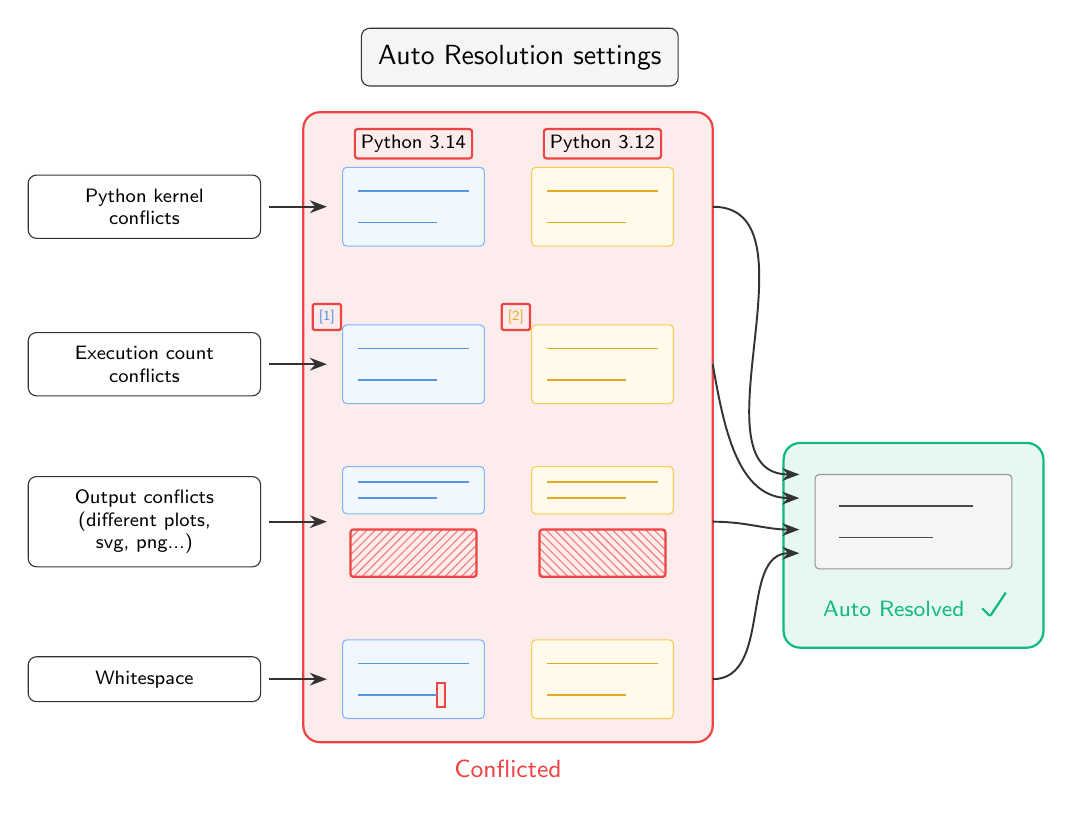
\begin{tikzpicture}[font=\sffamily\small, >=Stealth]

% Helper macro to draw straight "code" lines inside cells
\newcommand{\codeline}[3]{
    \draw[#1, line width=0.6pt] (#2) -- (#3);
}

%%=============================================================
%% BACKGROUND HIGHLIGHTS (Conflicted & Resolved Areas)
%%=============================================================
% Conflicted Background (drawn first to be at the back)
\draw[errRed, thick, fill=errRed!10, rounded corners=6pt] (3.5, -0.8) rectangle (8.7, 7.2);
\node[font=\sffamily\small, text=errRed, anchor=north] at (6.1, -0.9) {Conflicted};

% Auto Resolved Background (drawn first to be at the back)
\draw[resGreen, thick, fill=resGreen!10, rounded corners=6pt] (9.6, 0.4) rectangle (12.9, 3.0);

%%=============================================================
%% TOP TITLE
%%=============================================================
\node[draw=black!80, fill=cellBg, rounded corners=3pt, font=\sffamily, inner sep=6pt, anchor=center] 
    at (6.25, 7.9) {Auto Resolution settings};

%%=============================================================
%% LEFT COLUMN: SETTING LABELS
%%=============================================================
\tikzset{
    setting/.style={draw=black!80, fill=white, rounded corners=3pt, font=\sffamily\scriptsize, 
                    inner sep=5pt, align=center, text width=2.6cm, anchor=west}
}

\node[setting] (l1) at (0, 6) {Python kernel\\conflicts};
\node[setting] (l2) at (0, 4) {Execution count\\conflicts};
\node[setting] (l3) at (0, 2) {Output conflicts\\(different plots, svg, png...)};
\node[setting] (l4) at (0, 0) {Whitespace};

% Arrows from labels to the cell column gap
\draw[->, black!80, line width=0.7pt] (l1.east) ++(0.1,0) -- (3.8, 6);
\draw[->, black!80, line width=0.7pt] (l2.east) ++(0.1,0) -- (3.8, 4);
\draw[->, black!80, line width=0.7pt] (l3.east) ++(0.1,0) -- (3.8, 2);
\draw[->, black!80, line width=0.7pt] (l4.east) ++(0.1,0) -- (3.8, 0);

%%=============================================================
%% MIDDLE COLUMNS: CONFLICTING CELLS
%%=============================================================

%% --- ROW 1: Kernel Conflicts ---
% Python version annotations
\node[font=\sffamily\scriptsize, text=black, inner sep=2pt] (py1) at (4.9, 6.8) {Python 3.14};
\draw[errRed, thick, rounded corners=1pt] (py1.south west) rectangle (py1.north east);

\node[font=\sffamily\scriptsize, text=black, inner sep=2pt] (py2) at (7.3, 6.8) {Python 3.12};
\draw[errRed, thick, rounded corners=1pt] (py2.south west) rectangle (py2.north east);

% Current Cell
\draw[fill=curBg!40, draw=curBdr!80, rounded corners=1.5pt] (4.0, 5.5) rectangle (5.8, 6.5);
\codeline{curBdr!90!black}{4.2, 6.2}{5.6, 6.2}
\codeline{curBdr!90!black}{4.2, 5.8}{5.2, 5.8}

% Incoming Cell
\draw[fill=incBg!40, draw=incBdr!80, rounded corners=1.5pt] (6.4, 5.5) rectangle (8.2, 6.5);
\codeline{incBdr!90!black}{6.6, 6.2}{8.0, 6.2}
\codeline{incBdr!90!black}{6.6, 5.8}{7.6, 5.8}

%% --- ROW 2: Execution Count Conflicts ---
% Execution count box (Moved top left outside of Current Cell to avoid arrow)
\node[font=\sffamily\tiny, text=curBdr!90!black, inner sep=2pt] (cx1) at (3.8, 4.6) {[1]};
\draw[errRed, thick, rounded corners=0.5pt] (cx1.south west) rectangle (cx1.north east);

% Execution count box (Moved top left outside of Incoming Cell)
\node[font=\sffamily\tiny, text=incBdr!90!black, inner sep=2pt] (cx2) at (6.2, 4.6) {[2]};
\draw[errRed, thick, rounded corners=0.5pt] (cx2.south west) rectangle (cx2.north east);

% Current Cell
\draw[fill=curBg!40, draw=curBdr!80, rounded corners=1.5pt] (4.0, 3.5) rectangle (5.8, 4.5);
\codeline{curBdr!90!black}{4.2, 4.2}{5.6, 4.2}
\codeline{curBdr!90!black}{4.2, 3.8}{5.2, 3.8}

% Incoming Cell
\draw[fill=incBg!40, draw=incBdr!80, rounded corners=1.5pt] (6.4, 3.5) rectangle (8.2, 4.5);
\codeline{incBdr!90!black}{6.6, 4.2}{8.0, 4.2}
\codeline{incBdr!90!black}{6.6, 3.8}{7.6, 3.8}

%% --- ROW 3: Output Conflicts ---
% Current Cell Code (separated from output)
\draw[fill=curBg!40, draw=curBdr!80, rounded corners=1.5pt] (4.0, 2.1) rectangle (5.8, 2.7);
\codeline{curBdr!90!black}{4.2, 2.5}{5.6, 2.5}
\codeline{curBdr!90!black}{4.2, 2.3}{5.2, 2.3}

% Current Cell Output Box
\draw[errRed, thick, rounded corners=1pt, fill=white, pattern=north east lines, pattern color=errRed!70] 
    (4.1, 1.3) rectangle (5.7, 1.9);

% Incoming Cell Code (separated from output)
\draw[fill=incBg!40, draw=incBdr!80, rounded corners=1.5pt] (6.4, 2.1) rectangle (8.2, 2.7);
\codeline{incBdr!90!black}{6.6, 2.5}{8.0, 2.5}
\codeline{incBdr!90!black}{6.6, 2.3}{7.6, 2.3}

% Incoming Cell Output Box
\draw[errRed, thick, rounded corners=1pt, fill=white, pattern=north west lines, pattern color=errRed!70] 
    (6.5, 1.3) rectangle (8.1, 1.9);

%% --- ROW 4: Whitespace ---
% Current Cell
\draw[fill=curBg!40, draw=curBdr!80, rounded corners=1.5pt] (4.0, -0.5) rectangle (5.8, 0.5);
% First line with Whitespace conflict box at the end
\draw[curBdr!90!black, line width=0.6pt] (4.2, 0.2) -- (5.6, 0.2);
\draw[errRed, thick, fill=errRed!10] (5.2, -0.05) rectangle (5.3, -0.35);
\codeline{curBdr!90!black}{4.2, -0.2}{5.2, -0.2}

% Incoming Cell
\draw[fill=incBg!40, draw=incBdr!80, rounded corners=1.5pt] (6.4, -0.5) rectangle (8.2, 0.5);
\codeline{incBdr!90!black}{6.6, 0.2}{8.0, 0.2}
\codeline{incBdr!90!black}{6.6, -0.2}{7.6, -0.2}

%%=============================================================
%% RIGHT COLUMN: MERGED RESOLVED CELL
%%=============================================================

% Arrows Converging to the Resolved Cell
\draw[->, black!80, line width=0.7pt] (8.7, 6.0) to[out=0, in=180] (9.8, 2.6); 
\draw[->, black!80, line width=0.7pt] (8.7, 4.0) to[out=-80, in=180] (9.8, 2.3); 
\draw[->, black!80, line width=0.7pt] (8.7, 2.0) to[out=0, in=180] (9.8, 1.9);
\draw[->, black!80, line width=0.7pt] (8.7, 0.0) to[out=0, in=180] (9.8, 1.6);

% Auto-Resolved Output Cell
\draw[fill=cellBg, draw=cellBdr!80!black, rounded corners=1.5pt] (10.0, 1.4) rectangle (12.5, 2.6);
\codeline{black!70}{10.3, 2.2}{12.0, 2.2}
\codeline{black!70}{10.3, 1.8}{11.5, 1.8}

% Auto Resolved Label with Checkmark
\node[font=\sffamily\footnotesize, text=resGreen] (ar) at (11.0, 0.9) {Auto Resolved};
\draw[resGreen, thick, rounded corners=0.5pt] 
    (ar.east) ++(0.1, 0) -- ++(0.1, -0.1) -- ++(0.2, 0.3);

\end{tikzpicture}
\end{document}